\documentclass{beamer}\usepackage[]{graphicx}\usepackage[]{color}
%% maxwidth is the original width if it is less than linewidth
%% otherwise use linewidth (to make sure the graphics do not exceed the margin)
\makeatletter
\def\maxwidth{ %
  \ifdim\Gin@nat@width>\linewidth
    \linewidth
  \else
    \Gin@nat@width
  \fi
}
\makeatother

\definecolor{fgcolor}{rgb}{0.345, 0.345, 0.345}
\newcommand{\hlnum}[1]{\textcolor[rgb]{0.686,0.059,0.569}{#1}}%
\newcommand{\hlstr}[1]{\textcolor[rgb]{0.192,0.494,0.8}{#1}}%
\newcommand{\hlcom}[1]{\textcolor[rgb]{0.678,0.584,0.686}{\textit{#1}}}%
\newcommand{\hlopt}[1]{\textcolor[rgb]{0,0,0}{#1}}%
\newcommand{\hlstd}[1]{\textcolor[rgb]{0.345,0.345,0.345}{#1}}%
\newcommand{\hlkwa}[1]{\textcolor[rgb]{0.161,0.373,0.58}{\textbf{#1}}}%
\newcommand{\hlkwb}[1]{\textcolor[rgb]{0.69,0.353,0.396}{#1}}%
\newcommand{\hlkwc}[1]{\textcolor[rgb]{0.333,0.667,0.333}{#1}}%
\newcommand{\hlkwd}[1]{\textcolor[rgb]{0.737,0.353,0.396}{\textbf{#1}}}%
\let\hlipl\hlkwb

\usepackage{framed}
\makeatletter
\newenvironment{kframe}{%
 \def\at@end@of@kframe{}%
 \ifinner\ifhmode%
  \def\at@end@of@kframe{\end{minipage}}%
  \begin{minipage}{\columnwidth}%
 \fi\fi%
 \def\FrameCommand##1{\hskip\@totalleftmargin \hskip-\fboxsep
 \colorbox{shadecolor}{##1}\hskip-\fboxsep
     % There is no \\@totalrightmargin, so:
     \hskip-\linewidth \hskip-\@totalleftmargin \hskip\columnwidth}%
 \MakeFramed {\advance\hsize-\width
   \@totalleftmargin\z@ \linewidth\hsize
   \@setminipage}}%
 {\par\unskip\endMakeFramed%
 \at@end@of@kframe}
\makeatother

\definecolor{shadecolor}{rgb}{.97, .97, .97}
\definecolor{messagecolor}{rgb}{0, 0, 0}
\definecolor{warningcolor}{rgb}{1, 0, 1}
\definecolor{errorcolor}{rgb}{1, 0, 0}
\newenvironment{knitrout}{}{} % an empty environment to be redefined in TeX

\usepackage{alltt}
\usepackage{standalone}
\standalonetrue
\ifstandalone
  \usepackage{../haziq_beamer}
  \addbibresource{../bib/phd-presentation-3.bib}
\fi





\IfFileExists{upquote.sty}{\usepackage{upquote}}{}
\begin{document}

\ifstandalone
  \section{Examples}
\fi

\subsection{Fisher's Iris data set}

\begin{frame}[fragile]{Fisher's Iris data set}
\begin{knitrout}\small
\definecolor{shadecolor}{rgb}{0.969, 0.969, 0.969}\color{fgcolor}

{\centering 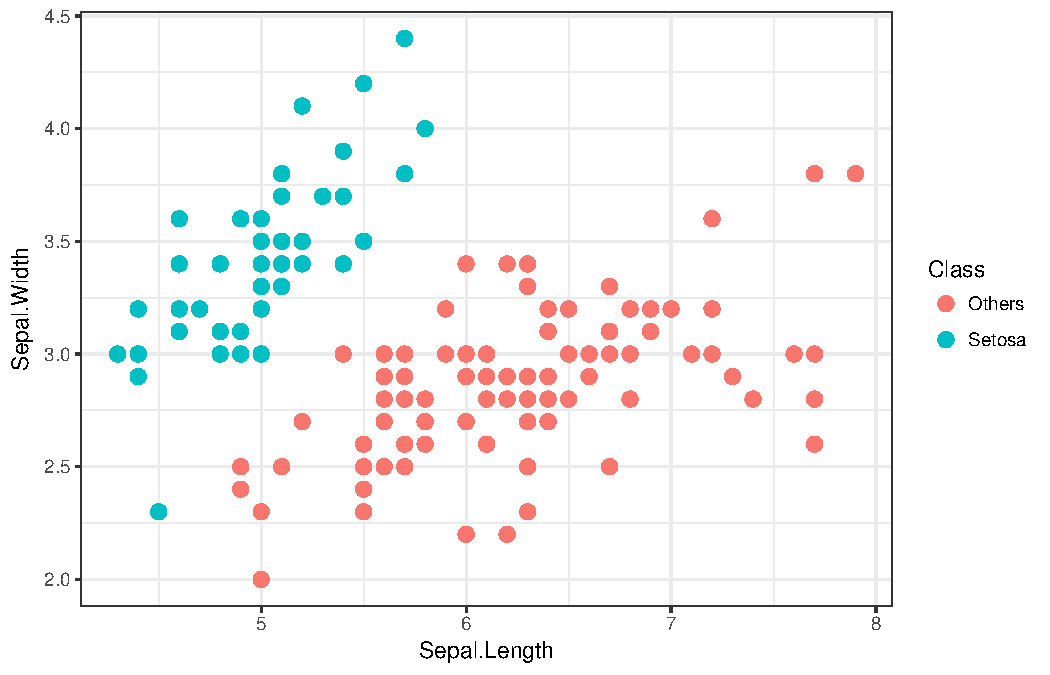
\includegraphics[width=\maxwidth]{figure/data_iris-1} 

}



\end{knitrout}
\end{frame}


\begin{frame}[fragile]{Fisher's Iris data set - Model fitting}
\blfootnote{\fullcite{Jamil2017iprobit}}
\vspace{-13pt}
\begin{itemize}
\item Varitional inference for I-prior probit models implemented in \proglang{R} package \pkg{iprobit} (still lots of work to do!).
\end{itemize}
\begin{knitrout}\small
\definecolor{shadecolor}{rgb}{0.969, 0.969, 0.969}\color{fgcolor}\begin{kframe}
\begin{alltt}
\hlstd{R> }\hlkwd{system.time}\hlstd{(}
\hlstd{+ }  \hlstd{(mod} \hlkwb{<-} \hlkwd{iprobit}\hlstd{(y, X))}
\hlstd{+ }\hlstd{)}
\end{alltt}
\end{kframe}
\end{knitrout}
\vspace{-25pt}
\begin{knitrout}\small
\definecolor{shadecolor}{rgb}{0.969, 0.969, 0.969}\color{fgcolor}\begin{kframe}
\begin{alltt}
\vspace{0.8em}
\end{alltt}
\end{kframe}
\end{knitrout}
\vspace{-25pt}
\begin{knitrout}\small
\definecolor{shadecolor}{rgb}{0.969, 0.969, 0.969}\color{fgcolor}\begin{kframe}
\begin{verbatim}
## 
## |=================================                     |  61%
##  Converged after 6141 iterations.
##  Training error rate: 0 %
##     user  system elapsed
##   67.857   6.396  74.277
\end{verbatim}
\end{kframe}
\end{knitrout}

\end{frame}

\begin{frame}[fragile]{Fisher's Iris data set - Model summary}
\begin{knitrout}\small
\definecolor{shadecolor}{rgb}{0.969, 0.969, 0.969}\color{fgcolor}\begin{kframe}
\begin{alltt}
\hlstd{R> }\hlkwd{summary}\hlstd{(mod)}
\end{alltt}
\begin{verbatim}
## 
## Call:
## iprobit(y = y, X, maxit = 10000)
## 
## RKHS used: Canonical 
## 
##           Mean   S.E.    2.5%   97.5%
## alpha  -4.1730 0.0816 -4.3330 -4.0129
## lambda  1.2896 0.0142  1.2618  1.3175
## 
## Converged to within 1e-05 tolerance. No. of iterations: 6141
## Model classification error rate (%): 0
## Variational lower bound: -12.93486
\end{verbatim}
\end{kframe}
\end{knitrout}
\end{frame}

\begin{frame}[fragile]{Fisher's Iris data set - Lower bound}
\vspace{-7pt}
\begin{knitrout}\small
\definecolor{shadecolor}{rgb}{0.969, 0.969, 0.969}\color{fgcolor}\begin{kframe}
\begin{alltt}
\hlstd{R> }\hlkwd{iplot_lb}\hlstd{(mod,} \hlkwc{niter.plot} \hlstd{=} \hlnum{10}\hlstd{)}
\end{alltt}
\end{kframe}
\end{knitrout}
\begin{knitrout}\small
\definecolor{shadecolor}{rgb}{0.969, 0.969, 0.969}\color{fgcolor}

{\centering 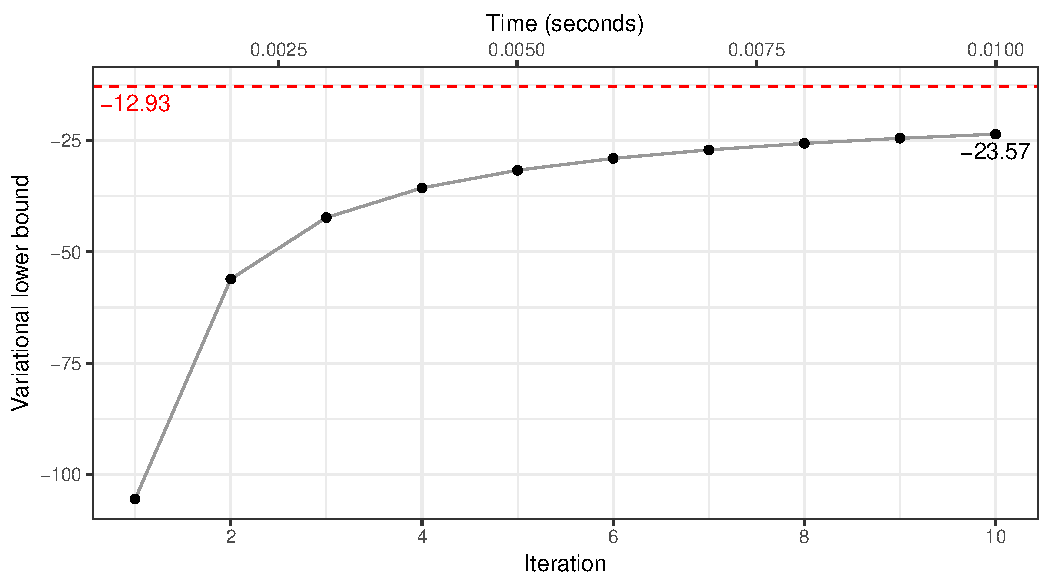
\includegraphics[width=\maxwidth]{figure/iris-lb-1} 

}



\end{knitrout}
\end{frame}

\begin{frame}[fragile]{Fisher's Iris data set - Decision boundary}
\vspace{-5pt}
\begin{knitrout}\small
\definecolor{shadecolor}{rgb}{0.969, 0.969, 0.969}\color{fgcolor}\begin{kframe}
\begin{alltt}
\hlstd{R> }\hlkwd{iplot_decbound}\hlstd{(mod)}
\end{alltt}
\end{kframe}

{\centering 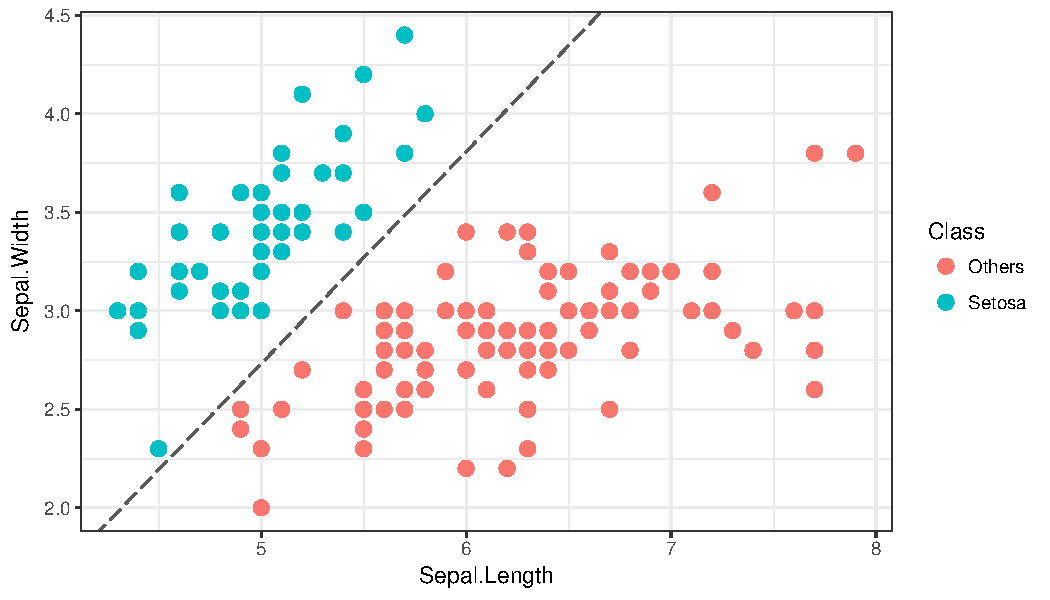
\includegraphics[width=\maxwidth]{figure/iris-decbound-1} 

}



\end{knitrout}
\end{frame}

\end{document}


